\section{Evaluatie}
\label{sec:eva}

Met een subsectie voor elke deelvraag.

In hoeverre is je vraag beantwoord?

Een mooie graphic/visualisatie is hier heel gewenst.

Hou het kort maar krachtig.


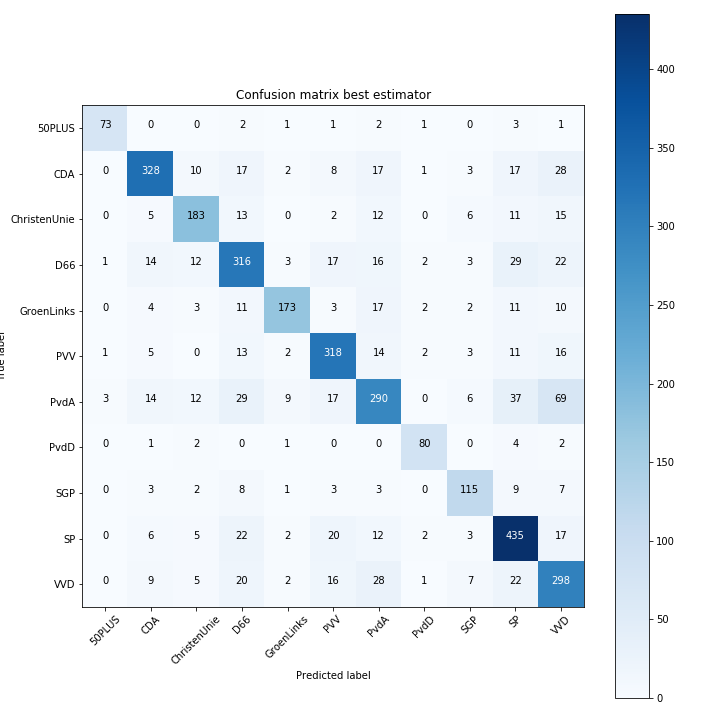
\includegraphics[width=0.6\paperwidth]{Verslag/confusionmatrix.png}

\subsection{Discussie}
\subsubsection{Deelvraag 1}
Dit onderzoek heeft zich beperkt tot methoden genoemd in eerdere onderzoeken én waarvan de implementatie beschikbaar is in Python. Een aantal methoden die in gerelateerde literatuur leidden tot goede classificaties zijn daarom niet getest. Ook nieuwe methoden die nog niet gebruikt zijn in een gepubliceerd artikel voor politieke tekst classificatie zijn daarom niet getest. Omdat niet alle opties getest zijn, kan geen uitsluitsel gegeven worden dat dit daadwerkelijk het classificatiemodel is. Voor vervolgonderzoek kan daarom gekeken worden om meer van deze methoden mee te nemen.\par

\subsubsection{Deelvraag 4}
Er zijn verschillende visies op links en rechts, en de indeling van de partijen, ook buiten de twee methoden gekozen in dit onderzoek.\par